\documentclass[tikz,border=10pt]{standalone}
\usepackage{amsmath}
\begin{document}

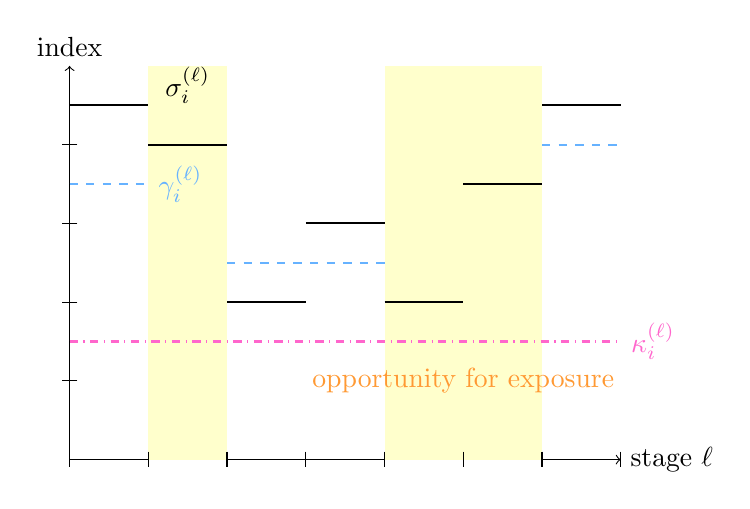
\begin{tikzpicture}
    % Colors
    \definecolor{exposureyellow}{RGB}{255, 255, 204}
    \definecolor{gammaBlue}{RGB}{102, 178, 255}
    \definecolor{kappaPink}{RGB}{255, 102, 204}
    \definecolor{opportunityOrange}{RGB}{255, 153, 51}
    
    % Axes
    \draw[->] (0,0) -- (7,0) node[right] {stage $\ell$};
    \draw[->] (0,0) -- (0,5) node[above] {index};
    
    % Yellow regions for opportunities
    \fill[exposureyellow] (1,0) rectangle (2,5);
    \fill[exposureyellow] (4,0) rectangle (6,5);
    
    % Gamma_i^(\ell) and Kappa_i^(\ell) lines
    \draw[dashed, thick, gammaBlue] (0,3.5) -- (1,3.5) node[right] {$\gamma_i^{(\ell)}$};
    \draw[dashed, thick, gammaBlue] (2,2.5) -- (4,2.5);
    \draw[dashed, thick, gammaBlue] (6,4) -- (7,4);
    
    \draw[dash dot, thick, kappaPink] (0,1.5) -- (7,1.5) node[right] {$\kappa_i^{(\ell)}$};
    
    % Index steps
    \draw[thick] (0,4.5) -- (1,4.5);
    \draw[thick] (1,4) -- (2,4);
    \draw[thick] (2,2) -- (3,2);
    \draw[thick] (3,3) -- (4,3);
    \draw[thick] (4,2) -- (5,2);
    \draw[thick] (5,3.5) -- (6,3.5);
    \draw[thick] (6,4.5) -- (7,4.5);
    
    % Index labels
    \node at (1.5,4.75) {$\sigma_i^{(\ell)}$};
    
    % Opportunity for exposure label
    \node[opportunityOrange] at (5,1) {opportunity for exposure};
    
    % Add some ticks on x-axis
    \foreach \x in {0,1,2,3,4,5,6,7}
        \draw (\x,0.1) -- (\x,-0.1);
    
    % Add some ticks on y-axis
    \foreach \y in {1,2,3,4}
        \draw (0.1,\y) -- (-0.1,\y);

\end{tikzpicture}

\end{document}